\section{Compatible-prior experiments and an exact Bayes benchmark}\label{sec:bayes-experiment-details}
\subsection{The common environment and the schedule comparison}
The multiscale schedules have $k_j=2\cdot4^j$ competitors with lifetime $H_j=T/4^j$. Put $v_j=\sqrt{(k_j-1)/H_j}$ and $\epsilon_j=av_j/32$, where $a\in\{1,4,8\}$. For the simulated ranges $v_j\le1$, consecutive $v_j$ increase by more than a factor of two, and all dyadic exponents have the same parity. Every group is consequently retained by the selection in Section~\ref{S-sec:spectral-proofs} of the mathematical supplement. The reference has mean $\theta_j=1/2+\sum_{r<j}\epsilon_r$. Under the group's null all $k_j-1$ candidates have mean $\theta_j-\epsilon_j$; a spike replaces one such mean by $\theta_j+\epsilon_j$. The null has probability $1/2$ and each spike has probability $1/\{2(k_j-1)\}$. These latent draws are independent across groups. The anchor mean is $1/2$ and unused arms have mean $1/4$.

For each group the largest possible earlier mean is at most $\theta_j$, irrespective of the earlier latent draws. Reference levels are deterministic, so their observations do not reveal other groups' latent variables. In every simulated configuration, including $a=8$, all means are strictly between zero and one. The original lower-bound information calculation applies with $a=1$; the larger multipliers are sensitivity experiments on valid stationary environments, without the same claimed information constant.

The compressed schedule puts the first $2L$ competing labels at time one and all remaining labels at time $T$. Its native prior is constructed by the same selection rule, leaving its last-round arms at mean $1/4$. Each pair has the same label set and tie ordering. At $a=4$, every mean vector from either native prior is evaluated on both schedules. Labels and means remain fixed during this crossing; only arrival times change. Native-prior comparisons and crossed comparisons therefore answer different questions. Other gap multipliers are evaluated only on their native schedules.

Each of the 23,552 trajectories uses a causal policy. MC-MOSS and Cold MC share local clock, frozen capacity, and smallest-label ties; Cold MC alone clears its counts and sums when the competitor count doubles. Both see only observed arrivals and rewards. The simulator supplies one independent uniform variate per calendar round, shared across the two methods and across receiving schedules for a fixed environment. Distinct replications use independent seed sequences. The simulation comprises 591,134,720 policy rounds. Each window is the native testing window of the receiving schedule. Windows are disjoint; their losses and the loss outside their union sum to the full trajectory loss. At $T=65536$, $L=4$ and $a=4$, the four native multiscale windows contribute 3.87, 9.59, 13.75 and 15.39 units of mean MC-MOSS regret, with 104.07 outside their union.

\begin{figure}[tb]
 \centering
 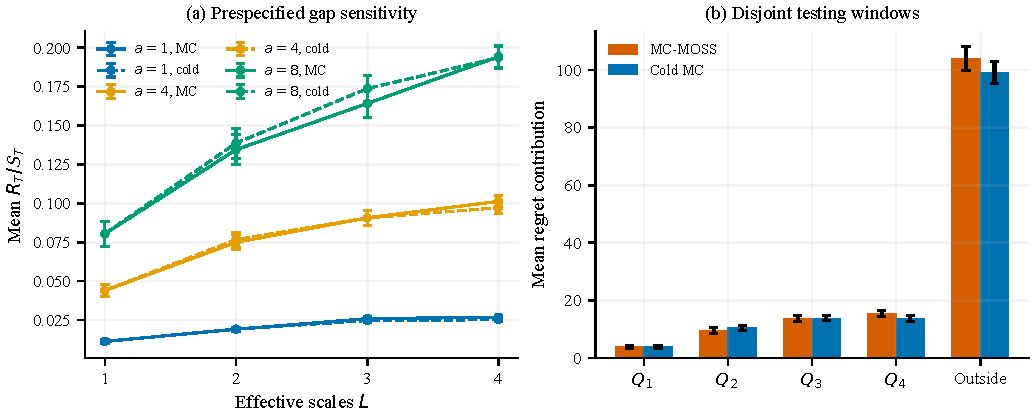
\includegraphics[width=\textwidth]{figures_v2/fig_geometry_sensitivity.pdf}
 \caption{Prespecified sensitivity and window losses at $T=65536$. Left: spectral-normalized native-prior risk for multipliers $a=1,4,8$. Right: regret in the four disjoint testing windows and outside their union for $L=4$, $a=4$. Error bars are $1.96$ Monte Carlo standard errors across 128 independent replications. The proof's small gap constant produces small absolute losses; increasing it changes finite-sample difficulty without changing the spectrum.}
 \label{fig:geometry-sensitivity}
\end{figure}

\subsection{An exact finite-prior dynamic program}
Let $\{\mu^{(e)}:e\in E\}$ be a finite set of Bernoulli mean vectors with strictly positive rational coordinates below one, and let $w_e>0$ be rational prior weights summing to one. The deterministic schedule and this prior are known to the Bayes rule. For every uncertain arm, retain its numbers of successes and failures in a state $s$. Arms whose mean is identical in all environments need not enter $s$. The posterior is
\[
 p_e(s)=\frac{w_e\prod_i (\mu_i^{(e)})^{s_i^+}(1-\mu_i^{(e)})^{s_i^-}}
 {\sum_f w_f\prod_i (\mu_i^{(f)})^{s_i^+}(1-\mu_i^{(f)})^{s_i^-}}.
\]
Action probabilities cancel from the likelihood because the decision rule is the same function of past observations in every environment. This remains true for adaptive sampling. Define
\[
 q_i(s)=\sum_ep_e(s)\mu_i^{(e)},\qquad
 g_t(i,s)=\sum_ep_e(s)\left(\max_{a\in A_t}\mu_a^{(e)}-\mu_i^{(e)}\right).
\]
Write $s^{i,y}$ for the updated state after reward $y$, and leave the state unchanged when $i$ has a known mean. The terminal value is $V_{T+1}=0$, and backward induction gives
\begin{equation}\label{eq:finite-bayes-recursion}
 V_t(s)=\min_{i\in A_t}\{g_t(i,s)+q_i(s)V_{t+1}(s^{i,1})+
       [1-q_i(s)]V_{t+1}(s^{i,0})\}.
\end{equation}

\begin{proposition}\label{prop:exact-finite-bayes}
The recursion \eqref{eq:finite-bayes-recursion} equals the minimum Bayes expected pseudo-regret over all causal policies with the specified information. All its entries are rational, and its initial value is a lower bound for the deterministic-schedule minimax regret over bounded stationary reward laws.
\end{proposition}
\begin{proof}
The posterior is sufficient for prediction because rewards are independent conditional on the environment and the observed counts determine the likelihood. Given the state and selected arm, the next reward is Bernoulli with mean $q_i(s)$, and its conditional expected current regret is $g_t(i,s)$. At the final round minimizing that expectation is optimal. Induction on the number of remaining rounds gives \eqref{eq:finite-bayes-recursion}; randomization cannot improve the minimum of finitely many action values. There are finitely many states with at most $T$ observations, and all posterior denominators are positive. Sums, products, ratios and finite minima of rational numbers remain rational, so exact arithmetic computes the value without rounding an action comparison. Finally, for every policy the supremum over reward laws is at least its average over this finite prior. Taking the infimum over policies proves the lower-bound assertion. Allowing the optimizing policy to use this known prior gives precisely the infimum of that average, not a larger quantity.
\end{proof}

We use six arms with arrivals $(1,1,1,T-1,T-1,T-1)$, for $T\in\{4,6,8,10\}$. Labels in this description start at zero. The anchor and the first reference (labels 0 and 1) have mean $1/2$; label 2 has mean $1/2-\epsilon_1$ or $1/2+\epsilon_1$, with equal probability. Label 3 has mean $1/2+\epsilon_1$. Labels 4 and 5 have common null mean $1/2+\epsilon_1-\epsilon_2$ with probability $1/2$; with probability $1/4$ each, one of them alone has mean $1/2+\epsilon_1+\epsilon_2$. The two latent draws are independent, giving six environments. We set $(\epsilon_1,\epsilon_2)=(1/d,2/d)$ for $d=16,8$. This small example retains the common null/spike structure; it is not an attempt to reproduce all dyadic testing-window conditions at these very short horizons.

All Bellman probabilities, values and comparisons are computed as exact fractions. We independently integrate the returned optimal rule over each environment's complete binary reward tree; the weighted average agrees exactly with the initial Bellman value in all eight cases. The risks of the two implemented anytime policies are computed by the same full reward-tree integration, retaining each policy's full observation history. Their index decisions use the stated numerical implementation. No Monte Carlo approximation enters this benchmark.

\begin{table}[tb]
\centering
\caption{Exact finite-prior risks, displayed to six decimals. The optimal rule knows the prior and complete schedule; MC-MOSS and Cold MC do not. Exact numerators and denominators are supplied with the code.}
\label{tab:exact-bayes}
\begin{tabular}{rr rrr}
\toprule
$T$ & $d$ & Bayes optimum & MC-MOSS & Cold MC\\
\midrule
4 &16&0.183594&0.250000&0.312500\\
6 &16&0.237320&0.311523&0.374023\\
8 &16&0.289612&0.368656&0.431156\\
10&16&0.339413&0.428149&0.490649\\
4 &8 &0.359375&0.500000&0.625000\\
6 &8 &0.449463&0.621094&0.746094\\
8 &8 &0.534172&0.724670&0.849670\\
10&8 &0.610496&0.837447&0.962447\\
\bottomrule
\end{tabular}
\end{table}

\begin{figure}[tb]
 \centering
 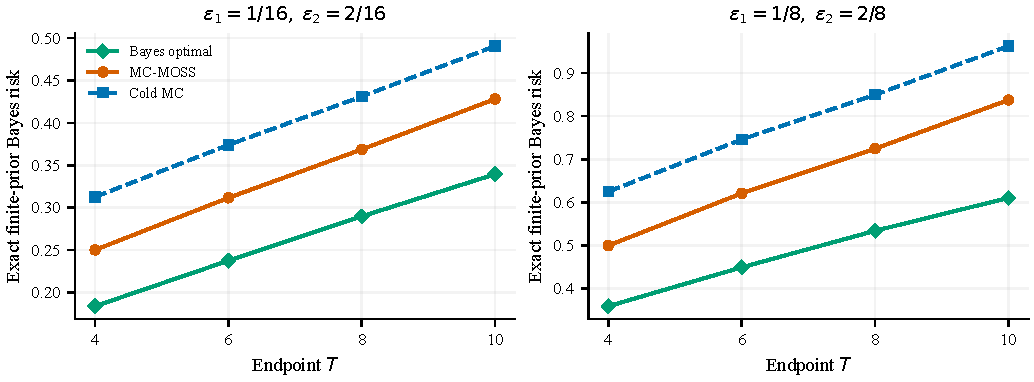
\includegraphics[width=\textwidth]{figures_v2/fig_bayes_exact.pdf}
 \caption{Exact finite-prior Bayes risks for the two gap choices. The green curve is the value of a rule with known schedule and prior. It is a certified lower bound, with no claim that this prior is least favorable. All plotted values are exact rational calculations, so there are no Monte Carlo error bars.}
 \label{fig:bayes-exact}
\end{figure}
